% Producto cruz: C = A x B perpendicular al plano de A y B (libro fig. 1.4)
\documentclass[border=4pt]{standalone}
\usepackage{tikz}
\usetikzlibrary{arrows.meta, calc}
\begin{document}
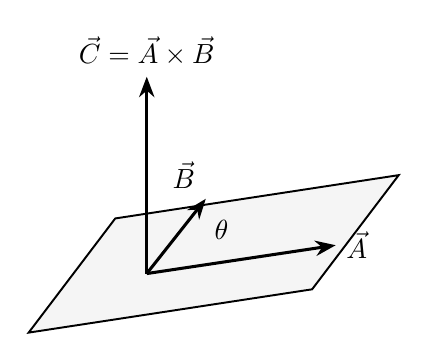
\begin{tikzpicture}[>={Stealth[length=2.6mm]}, line width=0.7pt]
  % plano de A y B (paralelogramo en perspectiva)
  \fill[black!4] (0,0) -- (3.6,0.55) -- (4.7,2.0) -- (1.1,1.45) -- cycle;
  \draw (0,0) -- (3.6,0.55) -- (4.7,2.0) -- (1.1,1.45) -- cycle;
  \coordinate (O) at (1.5,0.75);
  \draw[->, line width=1.1pt] (O) -- ($(O)+(2.4,0.36)$) node[right]{$\vec A$};
  \draw[->, line width=1.1pt] (O) -- ($(O)+(0.75,0.95)$) node[above left]{$\vec B$};
  \draw[->, line width=1.1pt] (O) -- ($(O)+(0,2.5)$) node[above]{$\vec C=\vec A\times\vec B$};
  \node at ($(O)+(0.95,0.55)$) {$\theta$};
\end{tikzpicture}
\end{document}
